\documentclass{article}
\usepackage{graphicx}

\title{Unstructured Information Processing 3}
\author{Divij Singh}
\date{23/09/19}


\begin{document}

\maketitle
	
\section{Q1}
For this assignment, I used Sklearn and Regular Expressions. I used the classified training and test data.\\
I split the data into training and testing lists, with the positive reviews first followed by the negative reviews for each.\\\\
I then used Sklearn to form a corpus from the entire training dataset, and converted the reviews into simple one-hot encodings (using unigrams). In the encoding, the presence of a word in a review was indicated by a 1 for true, and 0 for false. Using this, I used Sklearn to create and train a Logistic Regression model.\\\\
The resulting accuracy was 87.964\%, with 11,037 True Positives and 1,463 False Negatives

\section{Q2}
From the given data, we have the following:\\\\
States : Hot, Cold\\
Observations : 0, 1, 2 (Ice Creams Sold)\\\\
Starting Probability: \\$P(H) = 0.6$\\ $P(C) = 0.4$\\\\
Transition Probability: \\ $P(H|H) = 0.9$\\ $P(H|C) = 0.1$\\ $P(C|C) = 0.8$\\ $P(C|H) = 0.2$\\\\\\
Emission Probability: \\$P(H|0) = 0.14$\\$P(H|1) = 0.29$\\$P(H|2) = 0.57$\\$P(C|0) = 0.56$\\$P(C|1) = 0.34$\\$P(C|2) = 0.1$\\\\
All of this can be visualised as below:\\\\

\begin{figure}[h]
\caption{Starting and Transition Probabilities}
\centering
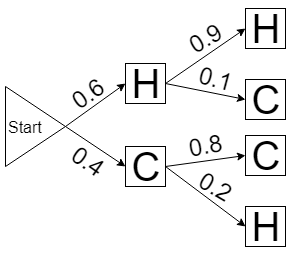
\includegraphics[width=0.5\textwidth]{Starting_and_Transition.png}
\end{figure}
\begin{figure}[h]
\caption{Emission Probabilities}
\centering
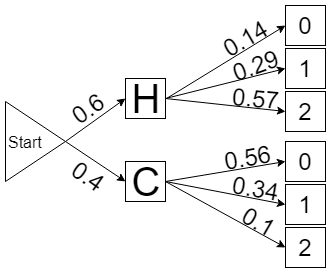
\includegraphics[width=0.5\textwidth]{Emission.png}
\end{figure}

\end{document}